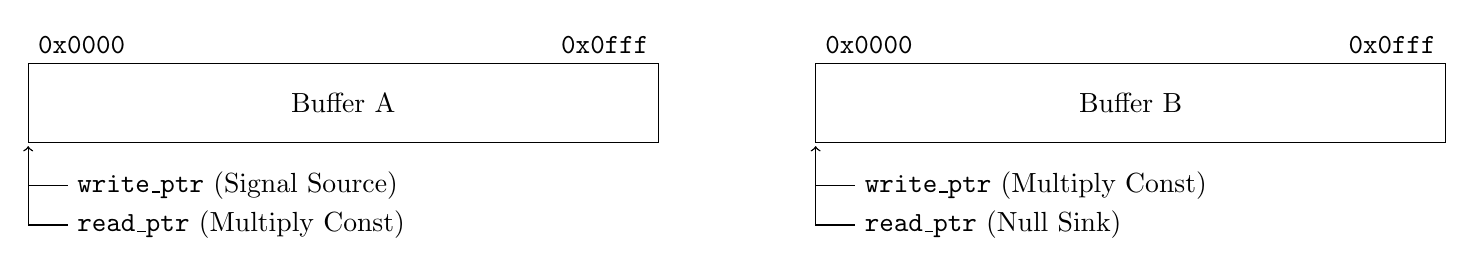
\begin{tikzpicture}
  \begin{scope}
    \draw
    (1, 4) rectangle (9, 5)
    (1, 5) node[anchor=south west]{\texttt{0x0000}}
    (9, 5) node[anchor=south east]{\texttt{0x0fff}}
    (5, 4.5) node[anchor=center]{Buffer A};

    \draw[<-]
    (1, 3.95) -- ++(0, -0.5) -- ++(0.5, 0) node[anchor=west]{\texttt{write\_ptr} (Signal Source)};

    \draw[<-]
    (1, 3.95) -- ++(0, -1) -- ++(0.5, 0) node[anchor=west]{\texttt{read\_ptr} (Multiply Const)};
  \end{scope}

  \begin{scope}[shift={(10, 0)}]
    \draw
    (1, 4) rectangle (9, 5)
    (1, 5) node[anchor=south west]{\texttt{0x0000}}
    (9, 5) node[anchor=south east]{\texttt{0x0fff}}
    (5, 4.5) node[anchor=center]{Buffer B};

    \draw[<-]
    (1, 3.95) -- ++(0, -0.5) -- ++(0.5, 0) node[anchor=west]{\texttt{write\_ptr} (Multiply Const)};

    \draw[<-]
    (1, 3.95) -- ++(0, -1) -- ++(0.5, 0) node[anchor=west]{\texttt{read\_ptr} (Null Sink)};
  \end{scope}
\end{tikzpicture}
